\documentclass[12pt]{article}
\usepackage[a4paper,top=16mm,bottom=16mm,left=17mm,right=17mm]{geometry}
\usepackage{fontspec}
\setmainfont{Times New Roman}
\usepackage{array}
\usepackage{booktabs}
\usepackage{amsmath}
\usepackage{enumitem}
\usepackage{xcolor}
\usepackage{fancyhdr}
\usepackage{hyperref}
\usepackage{tikz}
\usetikzlibrary{arrows.meta,positioning}

\definecolor{titleblue}{HTML}{183B56}
\definecolor{lightblue}{HTML}{EAF2F7}
\definecolor{linegray}{HTML}{66747D}
\hypersetup{colorlinks=true,urlcolor=titleblue,linkcolor=titleblue}
\setlength{\parindent}{0pt}
\setlength{\parskip}{4pt}
\setlist{leftmargin=1.45em,itemsep=2pt,topsep=3pt,parsep=0pt}
\renewcommand{\arraystretch}{1.13}
\pagestyle{fancy}
\fancyhf{}
\fancyfoot[L]{\small Team code: ST-77}
\fancyfoot[R]{\small Page \thepage\ of 5}
\renewcommand{\headrulewidth}{0pt}
\renewcommand{\footrulewidth}{0.3pt}
\newcommand{\tightsection}[1]{\vspace{2pt}{\large\color{titleblue}\bfseries #1}\par\vspace{1pt}}
\newcommand{\note}[1]{\colorbox{lightblue}{\parbox{0.955\linewidth}{#1}}}

\begin{document}

\begin{center}
{\LARGE\color{titleblue}\bfseries Design Details Document}\par
\vspace{3pt}
{\Large Autonomous Medical Supply and Quarantine Robot}\par
\vspace{4pt}
{\bfseries Robotics for Good Youth Challenge India 2026}\par
\vspace{2pt}
{\bfseries Team code: ST-77}
\end{center}

\tightsection{1. Clear understanding of the objective}

The challenge represents a public health emergency. The field includes healthcare centres and a quarantine area. Our robot focuses on two useful jobs. It delivers all ten medical kits in groups of 2, 6, and 2. It also carries and releases the two wooden beams used to close the quarantine zone. These jobs reduce repeated human contact with a risky area and move supplies where they are needed.

The robot must work by itself during the round. We place it in the starting area, switch it on, and press one start button. After that, the ESP32 controls every movement and release. The robot uses wall distance, a black tape marker, and fixed turn timing to follow a known route. It does not need a phone, laptop, remote control, or a person steering it.

The current 2026 rulebook gives a two-minute round and requires the robot to operate autonomously after activation. The complete robot, its ten kits, and its two beams must begin inside the $480 \times 280$ mm starting zone. Therefore, our main design goal is a compact and repeatable machine that completes selected scoring tasks within that time.

\tightsection{Tasks selected for this robot}

\begin{enumerate}
  \item Carry two kits to the first primary care centre.
  \item Carry six kits to the hospital area.
  \item Carry two kits to the second primary care centre.
  \item Carry two containment beams and release them at the quarantine area.
  \item Stop after the final release and wait for the end of the round.
\end{enumerate}

This version does not collect samples or sort the coloured triage cylinders. The rulebook allows teams to choose which actions they attempt. Hence, we kept the mechanism focused on kit delivery and beam placement.

\tightsection{Basic idea}

The robot uses differential drive. Two geared motors move it forward and turn it in place. Three gravity bins hold the kits. A small servo opens each bin flap once. Two more servo grippers hold the beams. The front ultrasonic sensor measures distance from a wall. Two downward-facing IR sensors detect a black tape crossing. This is actually a simple system, but each part has one clear job.

\note{\textbf{Submission configuration:} The robot starts with one pushbutton on ESP32 GPIO32. The selected program is \texttt{MinimalistCareBot.ino}. Once the button is pressed, it runs the full stored sequence without further input.}

\newpage
\tightsection{2. Description of the proposed mechanism}

\textbf{Overall size and estimated weight.} The design envelope is at most $460 \times 260$ mm so the loaded robot fits inside the $480 \times 280$ mm starting zone with a small placement margin. Height depends on the final bin and beam mounts. The estimated loaded mass is below 3.0 kg. The exact length, width, height, and mass will be measured after final assembly and checked before submission and inspection.

\textbf{Drive.} Two 12 V, 500 RPM geared DC motors drive one wheel on each side. A free caster supports the remaining end. The L298N driver changes motor direction and applies PWM speed control. Equal wheel commands move forward. Opposite wheel commands turn the robot on the spot.

\textbf{Kit mechanism.} Three separate bins are preloaded with 2, 6, and 2 wooden kits. Each kit is $25 \times 25 \times 20$ mm. The bottom of each bin has a flap. A positional servo opens the flap and gravity releases the complete group. Keeping the groups separate avoids counting kits during the run.

\textbf{Beam mechanism.} Two grippers carry the wooden containment beams. Each beam has a $60 \times 20$ mm section. One gripper is mounted for the first beam and one for the second. Each gripper has its own servo. The robot stops before every release, opens the correct gripper, and leaves it open so the beam can fall clear.

\textbf{Structure and materials.} A flat plywood, acrylic, or aluminium chassis can support the motors and electronics. Brackets hold the bins, sensors, and grippers. The bin walls may be plywood, acrylic sheet, or a light 3D-printed plastic. Rubber tyres provide grip. Screws and removable brackets make repairs easier.

\begin{center}
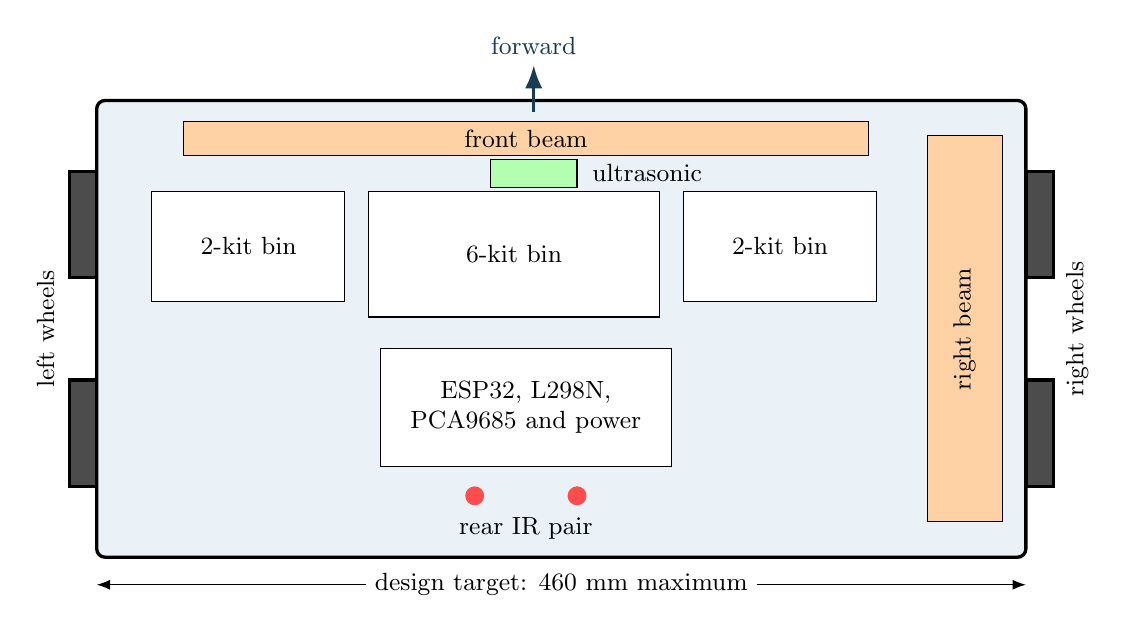
\begin{tikzpicture}[x=1cm,y=1cm,>=Latex,font=\small]
  \draw[very thick,rounded corners=3pt,fill=lightblue] (0,0) rectangle (11.8,5.8);
  \draw[very thick,fill=black!70] (-0.35,0.9) rectangle (0,2.25);
  \draw[very thick,fill=black!70] (-0.35,3.55) rectangle (0,4.9);
  \draw[very thick,fill=black!70] (11.8,0.9) rectangle (12.15,2.25);
  \draw[very thick,fill=black!70] (11.8,3.55) rectangle (12.15,4.9);
  \node[rotate=90] at (-0.65,2.9) {left wheels};
  \node[rotate=90] at (12.45,2.9) {right wheels};
  \draw[fill=white] (0.7,3.25) rectangle (3.15,4.65);
  \draw[fill=white] (3.45,3.05) rectangle (7.15,4.65);
  \draw[fill=white] (7.45,3.25) rectangle (9.9,4.65);
  \node at (1.93,3.95) {2-kit bin};
  \node at (5.30,3.85) {6-kit bin};
  \node at (8.68,3.95) {2-kit bin};
  \draw[fill=white] (3.6,1.15) rectangle (7.3,2.65);
  \node[align=center] at (5.45,1.90) {ESP32, L298N,\\PCA9685 and power};
  \draw[fill=orange!35] (10.55,0.45) rectangle (11.5,5.35);
  \node[rotate=90] at (11.02,2.9) {right beam};
  \draw[fill=orange!35] (1.1,5.10) rectangle (9.8,5.53);
  \node at (5.45,5.31) {front beam};
  \draw[fill=green!30] (5.0,4.70) rectangle (6.1,5.05);
  \node[right=2pt] at (6.1,4.88) {ultrasonic};
  \fill[red!70] (4.8,0.78) circle (0.12);
  \fill[red!70] (6.1,0.78) circle (0.12);
  \node[below=1pt] at (5.45,0.66) {rear IR pair};
  \draw[->,very thick,titleblue] (5.55,5.65) -- (5.55,6.25) node[above]{forward};
  \draw[<->] (0,-0.35) -- node[fill=white]{design target: 460 mm maximum} (11.8,-0.35);
\end{tikzpicture}

\textbf{Figure 1.} Simple top-view design. Final mounts will follow the measured chassis.
\end{center}

\newpage
\tightsection{3. Electronics, actuators, sensors, and power}

\begin{tabular}{@{}p{0.29\linewidth}p{0.08\linewidth}p{0.55\linewidth}@{}}
\toprule
Part & Qty. & Purpose \\
\midrule
ESP32-WROOM-32 DevKit & 1 & Runs the autonomous sequence and reads the sensors. \\
L298N motor driver & 1 & Controls direction and PWM for both motors. \\
12 V geared DC motor & 2 & Differential drive for forward motion and turns. \\
PCA9685 servo driver & 1 & Sends 50 Hz control pulses to five servos over I$^2$C. \\
Positional servo & 5 & Three bin flaps and two beam grippers. \\
Ultrasonic sensor & 1 & Measures the distance to a wall in front of the robot. \\
Digital IR sensor & 2 & Detects a black tape stripe under the rear of the robot. \\
Start pushbutton & 1 & Starts one autonomous run. \\
Main power switch & 1 & Provides an accessible physical stop. \\
\bottomrule
\end{tabular}

\tightsection{Wiring used by both programs}

\begin{tabular}{@{}p{0.16\linewidth}p{0.31\linewidth}p{0.43\linewidth}@{}}
\toprule
GPIO / channel & Connection & Job \\
\midrule
25, 26 & L298N IN1, IN2 & Left motor direction \\
27, 14 & L298N IN3, IN4 & Right motor direction \\
33, 17 & L298N ENA, ENB & Left and right motor PWM \\
23, 34 & Ultrasonic TRIG, ECHO & Wall-distance measurement \\
35, 16 & Left and right IR outputs & Black tape detection \\
21, 22 & PCA9685 SDA, SCL & Servo-driver I$^2$C link \\
32 & Pushbutton to ground & Start input with internal pull-up \\
PCA 0, 1, 2 & Three bin servos & 2-kit, 6-kit, and 2-kit release \\
PCA 3, 4 & Two beam servos & First and second beam release \\
\bottomrule
\end{tabular}

The PCA9685 logic supply, called VCC, connects to ESP32 3.3 V. Its V+ terminal takes a separate regulated servo supply. All grounds are joined. The servos must not be powered from the ESP32 3.3 V pin. If the ultrasonic ECHO output is 5 V, a 10 k$\Omega$ and 15 k$\Omega$ divider lowers it to about 3 V before GPIO34. GPIO34 and GPIO35 are input-only, which is suitable here.

\tightsection{Power source}

The motors use a motor-compatible battery supply through the L298N. The ESP32 uses its supported regulated input. The five servos use a regulated 5 to 6 V supply connected to PCA9685 V+. The final battery and regulator ratings depend on measured motor stall current and the current drawn by all loaded servos. Basically, every supply must handle the real peak current without resetting the ESP32 or slowing a servo.

\tightsection{Why these sensors were selected}

The route has walls at useful stopping points, so one ultrasonic sensor gives a direct distance reading. Black tape already marks the field, so two low-cost IR sensors can confirm a crossing. Both IR sensors must see black together. This reduces false detection when only one sensor passes over a side line. The robot uses the sensors as checkpoints instead of trying to calculate its exact position everywhere.

\note{The main power switch must be easy to reach and clearly marked. It is the physical emergency stop required for inspection. The Serial \texttt{x} command is useful during testing, but it is not a replacement for the switch.}

\newpage
\tightsection{4. Autonomous working and software}

The final submission program is written for Arduino-ESP32 and uses the Adafruit PWM Servo Driver library. On power-up, the motors stay off. The ESP32 starts the PCA9685 at address \texttt{0x40}, sets it to 50 Hz, and commands all five servos to their closed positions. The program then waits for the pushbutton.

\textbf{One button starts the complete route:}

\begin{enumerate}
  \item Drive forward until the ultrasonic reading is 20 cm or less.
  \item Stop, turn 90 degrees left, and open channel 0 to drop two kits.
  \item Drive forward until both IR sensors detect the next black tape stripe. Stop and open channel 1 to drop six kits.
  \item Continue until the next 20 cm wall reading. Stop and open channel 2 to drop the other two kits.
  \item Turn 90 degrees left and drive until the ultrasonic sensor again reads 20 cm or less.
  \item Stop, turn left, and open channel 3 to release the first beam.
  \item Turn left again and open channel 4 to release the second beam.
  \item Stop both motors and remain still. A reset is required before another run.
\end{enumerate}

The robot therefore works autonomously after a single button press. The sensors decide when forward legs end. A timed motor command makes each left turn. Servo releases happen only while the drive motors are stopped. A 25-second timeout limits each travel step. If the ultrasonic sensor loses its echo, if a wall appears before the tape marker, or if a step times out, the program stops the motors.

\tightsection{The two firmware files}

\begin{tabular}{@{}p{0.30\linewidth}p{0.62\linewidth}@{}}
\toprule
File & Behaviour \\
\midrule
\texttt{MinimalistCareBot.ino} & Autonomous after the GPIO32 button press. It follows the direct route above and releases the two beams after separate left turns. This is the submission configuration. \\
\texttt{CareBotESP32.ino} & Also autonomous after the GPIO32 button press. It adds startup checks, logging, button debounce, configurable outlet corrections, and extra fault handling. Its present route releases both beams together at one final stop. \\
\bottomrule
\end{tabular}

Only one sketch can be uploaded to the ESP32 at a time. Both sketches compile for the common 30-pin ESP32-WROOM-32 DevKit. Both wait for a button while holding the motors off. Both then run without steering or further button presses. For the submitted route, we will upload the minimalist file because its beam sequence matches our planned demonstration.

\tightsection{Control method}

The drive system has no wheel encoder or gyroscope. Therefore, the robot combines sensor stops with calibrated timing. Wall distance corrects the long forward legs. The black tape gives a middle checkpoint. Turn duration is measured on the loaded robot. This approach is easy to understand and repair, but tyre slip and battery level can change the result. We will tune it on the real field surface.

\newpage
\tightsection{5. Calculations and design justification}

\textbf{Motor command.} The minimalist program uses 8-bit PWM. A value of 102 gives
\[
\text{duty cycle}=\frac{102}{255}\times 100\%=40\%.
\]
A simple starting estimate for a 500 RPM motor is $500 \times 0.40 = 200$ RPM. Actual loaded speed will be lower and is not perfectly proportional to PWM. Hence, 102 is a calibration starting point, not a measured wheel speed.

If the measured wheel diameter is $D$ mm and loaded wheel speed is $n$ RPM, the forward speed is
\[
v=\frac{\pi Dn}{60}\ \text{mm/s}.
\]
For example, a 65 mm wheel at a true 200 RPM gives about 681 mm/s. We will measure the real value with the complete payload and adjust PWM if needed.

\textbf{Ultrasonic distance.} Sound travels about 0.0343 cm per microsecond. The pulse travels to the wall and back, so
\[
d=\frac{t\times0.0343}{2}\ \text{cm}.
\]
The program stops when $d\leq20$ cm. The measured distance is from the sensor face. Front overhang and wheel coasting must still be checked.

\textbf{Turn timing.} A left turn drives the wheels in opposite directions for 580 ms. We will place tape marks at the start and end angles, run at full payload, and adjust the time until ten repeated turns finish close to 90 degrees. The same surface and battery state will be used for the final test.

\textbf{Payload grouping.} Three bins contain $2+6+2=10$ kits, exactly matching the medical kit task. Separate servos make each drop independent. Five servo channels are enough because channels 0 to 2 control the bins and channels 3 to 4 control the beams.

\textbf{Fit check.} The target footprint of $460 \times 260$ mm leaves 20 mm in length and 20 mm in width inside the $480 \times 280$ mm starting zone. That is 10 mm clearance per side when centred. The final loaded robot and every carried item will be measured together.

\tightsection{Testing before submission}

\begin{itemize}
  \item Raise the wheels and confirm left and right motor direction.
  \item Test each empty servo mechanism, then repeat with the real load.
  \item Check both IR sensors on the field floor and black tape.
  \item Confirm the ultrasonic sensor sees the wall instead of the front beam.
  \item Measure the loaded footprint, height, mass, wheel diameter, turn time, and total route time.
  \item Run at least ten complete trials and record every missed stop or failed release.
  \item Check that both beams are fully released, stable, and clear of the robot.
\end{itemize}

The firmware has compiled successfully for the ESP32. Physical accuracy still depends on the measurements above. We will not treat a software build as proof of a successful field run.

\tightsection{References}

\begin{enumerate}[label={[\arabic*]}]
  \item IHFC, ``Robotics for Good Youth Challenge (RFGYC'26),'' \href{https://www.ihfc.co.in/important-announcements/robotics-for-good-youth-challenge-rfgyc26/}{official competition page}.
  \item Robotics for Good Youth Challenge, \emph{Rulebook 2026-2027}, supplied competition rulebook.
  \item IHFC, \emph{Design Document and Video Submission Template}, used for the required headings and page format, \href{https://www.ihfc.co.in/wp-content/uploads/2024/09/Design-and-video-Submission_Robotics-for-Good-Youth-Challenge.pdf}{reference PDF}.
\end{enumerate}

\end{document}
